\chapter{Sample Implementation}\label{chap:sample_app}

A sample toy application has been created to validate the Jester sensor and data fusion abstraction framework. It uses the LeapMotion Controller and the PrimeSense Carmine to allow the user to either deflect or delete balls with her character's hands as they fall from the sky. These two sensors were selected because they provide an overlap of data about the users skeleton as described at the beginning of chapter \ref{chap:api_des}. Properly fusing the data in this system will require a small modification of the default data fusion module in order to handle the hand orientation ambiguity. This section will discuss the implementation of the required sensor wrappers, data fusion modifications, and a sample filtering algorithm.

\section{Sensor Wrappers}

The LeapMotion Controller and the PrimeSense Carmine are manufactured by different companies and use completely different skeletal APIs. So, each needs its own wrapper implementation. Ideally, there would be a support community of VR enthusiasts that would create sensor wrappers for new hardware and provide them to others. However, that will not exist initially and the process of creating wrappers must be demonstrably simple. This section will cover the process for creating wrappers for the LeapMotion Controller and the PrimeSense Carmine.

\subsection{LeapMotion Controller}\label{sec:leap_impl}

The LeapMotion Controller is designed for hand and finger tracking and has a relatively short range and narrow field of view, but is capable of tracking with high precision. LeapMotion's API provides an interface for registering a callback function that is triggered when there is new information about the hands visible. The callback is called with a reference to the current captured frame. The frame provides an accessor to get a list of all of the hands that the Controller can resolve in the current frame. The Controller can track as many hands as can cleanly fit in its field of view. Each hand has an ID that is unique to that hand. However, if the Controller loses tracking of a hand it will assign it a new ID. Similarly, each hand has a list of fingers; each with a unique ID. The IDs are assigned randomly and the API does not provide a guess about which finger is which. So, it is left to the developer to best decide how to resolve hand and finger identity.

This thesis resolves right and left hand position using a set of assumptions that must be followed for correct system behavior:

\begin{enumerate}
	\item There will never be more than 2 hands in the Controller's tracking space.
	\item If only one hand is inserted into the tracking space it is the left hand if it is to the left of the center of the Controller, and the right if it is to the right. This only holds true when the hand is first seen. Once that hand's ID is assigned it can move to either side of the Controller freely.
	\item If one hand is being tracked, the next hand that the Controller tracks is assigned to be the other.
\end{enumerate}

These rules have been experimentally determined to be effective most of the time. However, it is possible for the Controller to become confused and swap the hands it is tracking. The hands can be reset by withdrawing them from the tracking space, waiting a second, and then reinserting.

\begin{figure}[]
\centering
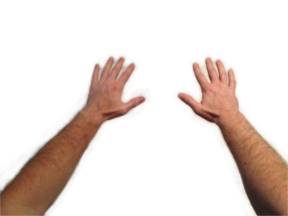
\includegraphics[width=0.5\textwidth]{figures/handsStraight}
\caption{The user's hands must be placed in front of the LeapMotion Controller with palms down and fingers spread in order to calibrate.}
\label{fig:hand_default}
\end{figure}

Finger tracking in the Leap is a bit more complex. Using the X-axis position of the fingers is unreliable in situations where the hands are rotated so that the fingers are pointing outward. The Controller API attempts to provide a vector that points along the hand direction, but it is unreliable. This thesis's implementation uses a calibration pose to solve the finger ambiguity issue. The wrapper waits until all five fingers are visible on the hand, and then assumes that the thumb is the inside finger along the X-axis and the rest of the fingers are placed normally with respect to that orientation as shown in figure \ref{fig:hand_default}. It then retrieves the length of each finger from the LeapMotion API and assigns it to that hand for the rest of that hand IDs life. Next, it gets the finger IDs from the API and assigns them in the same manner. Whenever a finger ID is lost, the wrapper stops reporting information about that finger. When an unknown finger ID is attached to the hand, the wrapper finds the finger on the hand that is not currently being tracked and has the closest length to the new finger. The new finger's ID is then assigned to that finger. This process is detailed in figure \ref{fig:finger_matching}. 

\begin{figure}[]
\centering
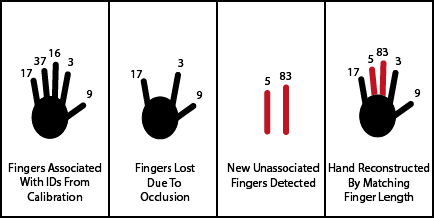
\includegraphics[width=.75\textwidth]{figures/fingerAssociation}
\caption{Finger IDs frequently become lost and must be reacquired using the calibrated length.}
\label{fig:finger_matching}
\end{figure}

Once the wrapper has calibrated finger length it begins to provide data about finger position. The LeapMotion Controller tracks finger tip position and orientation. Jester stores finger position using the knuckle joint and an imaginary joint placed at the end of the finger. The wrapper converts Controller finger data to Jester finger data by using the tip position as the imaginary end joint and estimating the position of the knuckle joint by moving backwards along the tip vector by the length of the finger.

The wrapper processes all of the hand and finger data that it can glean from the LeapMotion API on each invocation of the new frame callback. Once it has the LeapMotion objects for hands and fingers mapped, it translates the positions from LeapMotion points into GLM points and calls the controller's suggestJointInfo(...) method to pass it into the data fuser.

\subsection{PrimeSense Carmine}\label{sec:carmine_impl}

The PrimeSense Carmine is designed for full body tracking and has both a longer range and wider field of view than the LeapMotion Controller. It uses a skeletal tracking API called NiTE that was designed for the Carmine by PrimeSense. NiTE is capable of tracking all of the Jester bones that the LeapMotion Controller is not. There is also a very close to 1:1 mapping from the joints that are tracked by NiTE and the Jester joints. The Carmine wrapper only has to infer the position of the imaginary joint at the top of the head to generate head orientation and the position of the root bone, since it is not actually present on a skeleton.

The wrapper is implemented by setting up a polling thread that is launched when the Carmine wrapper is started. The thread simply polls the Carmine every 100ms to get new frame data. It assumes that the first skeleton present, since the Carmine can track multiple skeletons, is the relevant skeleton and waits until NiTE recognizes a full lock on its joint positions. Once a full lock has been achieved it converts the NiTE joints into GLM joints, assumes the head is always pointing up and that the root bone is at the midpoint between the two hip joints, and calls the controller's suggestJointInfo(...) method to feed the skeleton to the data fuser.

\section{Fusion Implementation}\label{sec:fuser_impl}

The data fusion requirements for the sample application are very close to being in line with the default functionality. There just needs to be a method for disambiguating the hand orientation from the LeapMotion Controller. So, the sample data fuser simply extends the default fuser and overrides the DataFusionModule::newData(...) function. The new implementation simply checks if the wrist joints are known in the current skeletal frame. If they are, then it checks if the incoming wrist joints would be closer to the existing positions if the hands were swapped like in figure \ref{fig:hand_swap}. If the change in difference is larger than a threshold the fuser assumes that the hands need to be swapped. If the incoming data is from the LeapMotion controller, then it creates a new map where the hands and fingers are swapped and then invokes the superclasse's newData(...) function with the new map. In the case where the Leap's finger data has already been placed in the current skeletal frame, the data in the frame is swapped and then the superclass's newData(...) function is called with the unchanged map. This small set of modifications to the base fuser class show that small system modifications are easy in situations where a close to default behavior is desired.

\begin{figure}[]
\centering
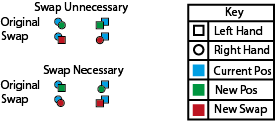
\includegraphics[width=0.5\textwidth]{figures/handSwap}
\caption{Hand position, represented as shapes, sometimes needs to be swapped due to data ambiguity.}
\label{fig:hand_swap}
\end{figure}

\section{Data Filtering}

The LeapMotion Controller provides very stable data, but the PrimeSense Carmine is prone to having joint positions suddenly "jump" from their correct location to a wildly incorrect position and then reset. So, the system stability can seriously benefit from filtering. This thesis implements a sample particle filter to attempt to reduce the system noise.

\subsection{Particle Filter}\label{sec:filter_impl}

A particle filter was selected because it is good for applications where a system dynamics model is difficult or impossible to create as discussed in section \ref{sec:filter_back}. The mathematical justification for particle filters is beyond the scope of this thesis, so only implementation level details will be discussed.

The first step in creating a particle filter is deciding what exactly the particles represent. In the example of skeletal tracking, they could either represent a guess at the state of the entire skeleton, or the state of one bone. The skeleton has too many degrees of freedom to be easily modelled in one particle, so each particle represents a guess at the position and orientation of a single bone. In practice, orientation has to be inferred later because quaternions can be interpolated, but there is not a good way to average large numbers of them together like there is for 3D position \cite{markley2007averaging}. So, each particle stores a bone start position and end position as 3D points. This means that there is a particle system for each bone in the Jester skeleton. When each particle system is generated, the particles represent random guesses at bone position. 

The update step in the particle filter needs some way to move the existing particles, or the filter would just stabilize and become static. So each particle also stores a movement direction vector and velocity for the endpoint. This allows the particles to simulate the rotation of the bone while avoiding the quaternion problem. On each pass through the filter, all of the particles have their endpoint moved in the direction vector by a distance calculated using the velocity and the time elapsed between updates.

After the update, the probability of each particle is calculated using the euclidean distance between the measured start and end points, calculated using the bone's orientation quaternion and the bone length, and the particles start and end points. Lower distance means that the particle is more likely. The resampling step generates a new particle using a selection wheel approach where the space occupied by a given particle on the circle is proportional to its probability. This method gives preference to more likely bone states, but still introduces mixed results to allow the filter to react to true changes quickly.

The filter then generates the bone's filtered position by calculating the statistical mean of the particle's start and end positions and creating a quaternion that represents the bone rotation formed by the vector from bone start to bone end. The filter returns the final new bone with the mean start position, the quaternion, and the length from the bone passed in as the update argument. 

\section{Sample Application}\label{sec:app_impl}

The sample application of Jester is mainly designed as a toy to prove that the concept of a sensor abstraction and data fusion framework can be useful. It is only vaguely useful and is only designed to showcase the cooperation between the PrimeSense Carmine and the LeapMotion Controller. Balls slowly fall from the ceiling and can either be deflected away or deleted on contact depending on the user's hand orientation. A huge bulk of the code is devote to handling mouse events, setting up OpenGL, and the simple physics engine. The implementation of all of these tools is outside the scope of this thesis. Jester's setup and query steps can be represented in the following steps that map 1:1 to code:

\begin{enumerate}
  \item Construct Jester Controller with Data Fuser Factory
  \item Construct Sensor object
  \item Set sensor orientation
  \item Set sensor position
  \item Add sensor to fuser
  \item Repeat 2-5 for each sensor
  \item Start sensors
  \item Get the Scene object from the Controller
  \item Call Scene::refreshSkeleton()
  \item Query Scene for bone position to draw skeleton
\end{enumerate}

The fact that so little of the application code is dealing with sensors and raw sensor data is a signal of the value of the Jester abstraction framework.
